% Report of results from Ramsay simulation experiment
% David Lawrence Miller
% d.l.miller@bath.ac.uk

% Started : 29 October 2008

\documentclass[a4paper,10pt]{amsart}

% Load some packages
\usepackage{times, amsmath, amssymb, amsfonts, url, natbib, bm, rotating}

\usepackage{multirow}
\usepackage{graphicx}

% top matter
\title{a title}
\author{David Lawrence Miller}
\email{d.l.miller@bath.ac.uk}
\address{Mathematical Sciences, University of Bath, Bath, United Kingdom}

% Shortcuts
% Probability
\newcommand{\prob}[1]{\mathbb{P}\left[ #1 \right]}
% Hovitz-Thompson
\newcommand{\HT}{\hat{\tau}_{HT}}
% Schwarz-Christoffel
\newcommand{\sch}{Schwarz-Christoffel }
% fprime
\newcommand{\fprime}{f^\prime(z)}
% figure reference command
\newcommand{\fig}[1]{\emph{fig.} (\ref{#1})}
% figure reference command (start of sentance
\newcommand{\Fig}[1]{\emph{Fig.} (\ref{#1})}
% equation reference command
\newcommand{\eqn}[1]{\emph{eqn.} (\ref{#1})}
% phi inverse
\newcommand{\phiinv}{\phi^{-1}}
% use other phi
\renewcommand{\phi}{\varphi}




\begin{document}

% The abstract
\begin{abstract}
Smoothing over complex 2-D regions is difficult. Several approaches have been proposed including finite element analysis (Ramsay, 2002), within-area distance (Wang \& Ranalli, 2007) and recently soap film smoothing (Wood, Bravington \& Hedley, 2008.) Here I investigate an alternative method based on the Schwarz-Christoffel transform from complex analysis. This takes the region and ``morphs'' it to a rectangle or disk in a prescribed way. We may then smooth over the transformed area using penalized regression splines and transform this smooth back to the original domain in order to perform analysis. I explore the utility of this transform for both real and simulated data.
\end{abstract}


% New theorem for theorems
\newtheorem{thm}{Theorem}[section]

%New theorem for definitions
\newtheorem{defn}{Definition}[section]

\maketitle



\section{Ramsey's horseshoe}

\cite{ramsay} proposes a function which can be used to benchmark new approaches to 2-dimensional smoothing. The function takes the form of a horseshoe which is flat across the domain but ranges from $-4$ to $4$ along the domain's major axis. The so-called ``Ramsay horseshoe'' is shown in \fig{ramsayshorseshoe}.

The test function highlights a common problem in spatial smoothing: that of ``leakage''. When the problem is specified in Euclidean distance, the model thinks that the distance between the $-4$ and $4$ points of the horseshoe is the distance over the gap in between them, rather than the distance along the major axis of the shape. This causes the high density from one side to contaminate the other (or the low to contaminate the high.) It is easy to see that this causes bias in the estimation of the smooth.

\Fig{tpleakage} shows what happens when a thin plate spline is fitted to the horshoe with no information about the structure of the domain. Comparing the contour lines to those in the actual horseshoe, one can easily see that there is leakage.



\begin{figure}
\centering
% trim order l b r t
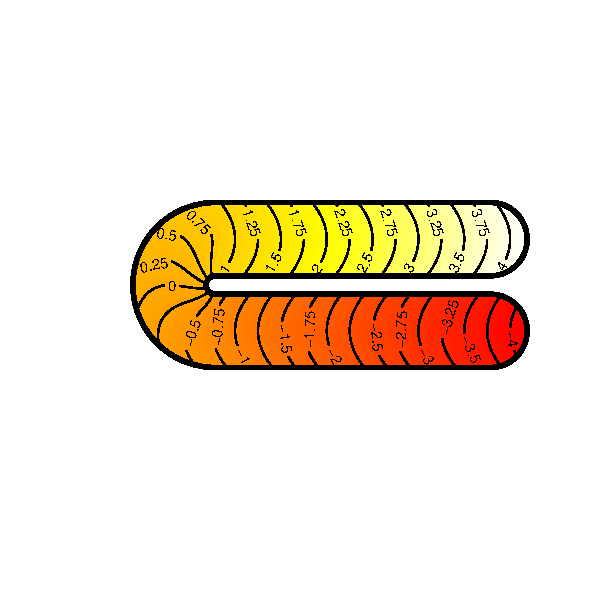
\includegraphics[trim=1.5in 1in 0.5in 1in]{figs/ramsayhorseshoe.pdf} \\
\caption{Heatmap of the Ramsay horseshoe.}
\label{ramsayshorseshoe}
\end{figure}

\begin{figure}
\centering
% trim order l b r t
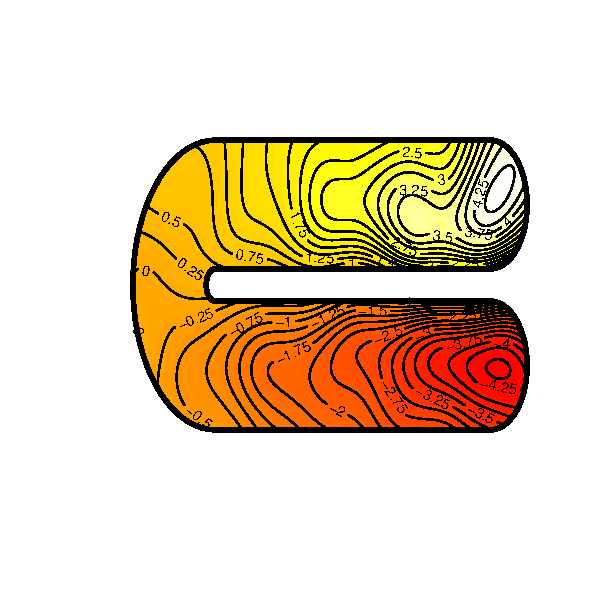
\includegraphics[trim=1.5in 1in 0.5in 1in]{figs/leakageexample.pdf} \\
\caption{An example of leakage when using a thin plate spline.}
\label{tpleakage}
\end{figure}

Clearly we would like to use an approach that respects the shape of the region and does not show any evidence of leakage. In order to deal with the problems of a complex region, four different approaches have been proposed:

\begin{enumerate}
\item \cite{ramsay} proposes finite area $L$-splines (FELSPLINEs.) The $L$-spline has a differential operator in its penalty, which cannot be analytically solved in two dimensions. However, to combat this, the author triangulates the domain and then constructs a set of bivariate quadratic polynomial basis functions over each triangle, specifying that there be continuity over the edges of the triangles. The union of these functions is then a solution to the PDE in the penalty and therefore the solution to the usual smoothing objective function\footnote{\emph{ie.} $\sum_{i=1}^n (z_i-f(x_i,y_i;\theta))^2 + \lambda \int_\Omega Pf(x,y;\theta)d\Omega$, where $P$  is the penalty in whatever form it takes.}.

FELSPLINE does not perform very well in practice since its boundary conditions specify that the gradient is normal to the edge of the area. This is not physically realistic in all situations.

\item \cite{wangranalli} adopt a ``within-area distance'' formulation for thin plate splines. In this case they take the geodesic distance between two points, that being the shortest path within the domain in order to address the problem of the definition of ``close'' in the domain. 

Since the geodesic distance is only known if the intrinsic structure of the domain is known (which is rare in ecological examples), the authors use a different method to calculate the shortest path. For this they create a graph of the data points, with nodes at each point and the linear interpolant between the nodes. Floyd's algorithm is then run to find the $k$ nearest neighbors of each node. Unfortunately this is $\mathcal{O}(N^3)$ if $N$ is the number of datum.


\item \cite{soap} consider a soap film over the domain which is weighed down by the data whilst minimizing the surface tension in the film.

\item An alternative approach is to ``morph'' the area in question to be one that is more suitable for smoothing upon. This is what we propose here. For example, with Ramsay's horseshoe, it seems intuitive to simply bend the horseshoe back to a long strip and then smooth on that domain.

This approach suffers from a few drawbacks. First, what is the natural domain to transform to? Clearly for some shapes this is obvious, but this is not always the case. The other problem is in fnding the nullspace of the smooth. It seems that the nullspace in the original domain will not be the same as the nullspace in the transformed domain. We address these problems below.


\end{enumerate}




\section{Method}

Here we formulate a conformal mapping from the domain of the problem (we call this the $W$ domain) to a domain on which it is easier to smooth (and where we can avoid the problems detailed above.) We elaborate on what was alluded to in \cite{eilerstalk}: using the \sch mapping to transform our domain to another in order to perform smoothing.

\subsection{\sch}

The \sch transform provides a way to map an arbitrary polygon in the complex plane to one of a set of objects (also in the complex plane) in a certain manner. The two most commonly mapped to objects are the unit disk and the rectangle. The procedure consists of adding vertices to the object you wish to map to and then deforming it iteratively until it is identical to the polygon.

So, for example, say we want to transform between a regular nonagon and a rectagle. We add five sides to the rectangle and then go about deforming it to the shape of the nonagon (by changing the angles at the vertices and then rescaling and rotating it as necessary.) 

Full technical details are given in \cite{miller08}.


\subsection{P-splines}
P-splines (\cite{eilersmarx96}) were used as the basis functions for the smooth since they present the easiest framework for adding arbitrary penalities. They are also not considered to be as ``optimal'' as thin plate splines.




\subsection{Procedure}

Our procedure consists of the following steps:

\begin{enumerate}
\item Determine the domain over which we would like to smooth, $W$.

\item Compute the \sch transform of $W$ to get $Z$.

\item Map the co-ordinates of the datapoints in $W$ to $Z$.

\item Fit the GAM to the data in $Z$.

\end{enumerate}

At this point it depends on the application as to whether a transform is needed to go back to the original domain. If we are only interested in, say, the density of a biological population, then this can be estimated in the transformed domain. On the other hand, it may be the objective to obtain other information of a graphical representation of the density, in which case the back-transform is required.



\subsection{Software}

There are several pieces of software available to perform the \sch mapping. The Fortran library \texttt{SCPACK} available on netlib was used initially, but only offers the mapping to the unit disk and does not include the CRDT method for performing the mapping (see \cite{miller08}, section BLAH.) For this reason the SC toolbox (\cite{driscoll}, SOME SECTION) for Matlab is used to perform the mapping. 

The \textsf{R} library \texttt{mgcv} provides subroutines for fitting generalized additive models and, in particular, P-splines.

There are packages available to enable \textsf{R} to talk to Matlab and vice-verse, however this seemed like overkill given the situation. So, for the purposes of this exploratory work csv files were written by each program and read in by the other.

\section{Mapping the Ramsay horseshoe}

In order to map the horseshoe, we draw a rough bounding box around the shape. This will serve as the domain that we want to transform from (rather than trying to approximate the curved edges with many straight lines.) The horseshoe, along with its bounding box is shown in \fig{hswithboundingbox}.

\begin{figure}
\centering
% trim order l b r t
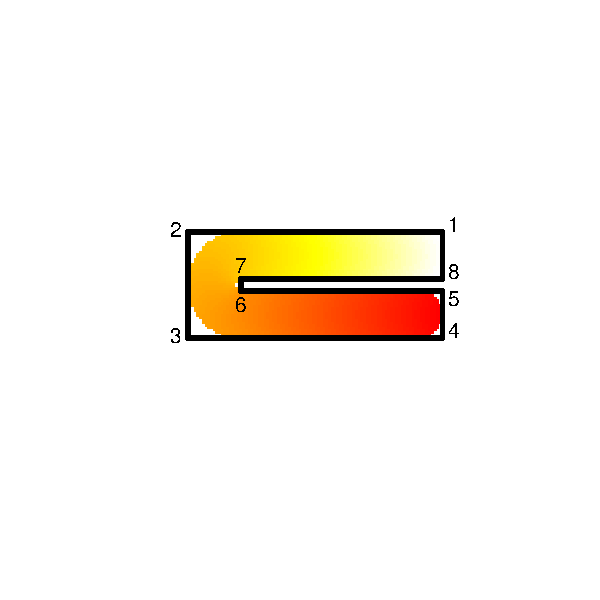
\includegraphics[trim=0in 1.5in 0in 1.5in]{figs/hswithboundingbox.pdf} \\
\caption{The horseshoe with it's bounding box. Vertices 1, 4, 5 and 8 are mapped to the corners of the rectangle.}
\label{hswithboundingbox}
\end{figure}

To begin with we took a sample of 1000 points from the horseshoe and then added some noise to the data. We then took the $x,y$ coordinates of the sampled points and ran them through the \texttt{evalinv()} function from the SC Toolbox. We then smoothed over the responses in the transformed domain. An example of the smooth is shown in \fig{examplescsmooth}.

Comparing \fig{examplescsmooth} with \fig{ramsayshorseshoe} we see that transforming the domain allows us to smooth over the horseshoe quite well. In the next section we investigate the properties of the transform further via a simulation experiment.



\begin{figure}
\centering
% trim order l b r t
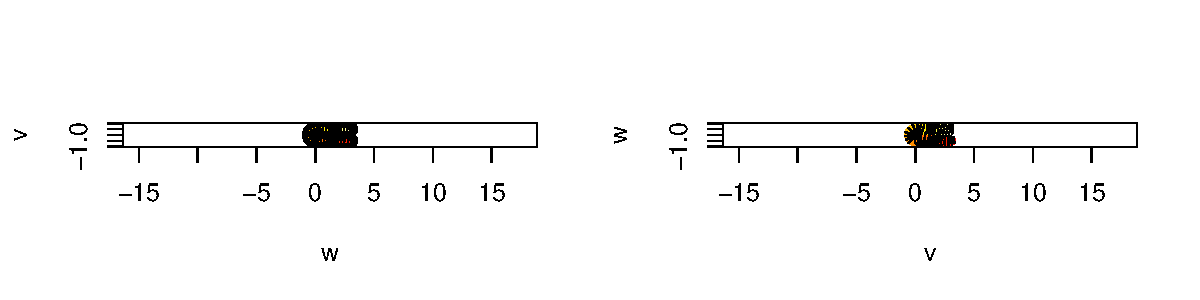
\includegraphics[trim=0in 1.5in 0in 1.5in]{figs/examplescsmooth.pdf} \\
\caption{An example of the smooth given with P-splines when the domain has been transformed using the \sch mapping.}
\label{examplescsmooth}
\end{figure}




Show the morphed region with heatmap and the prevertices on it!



\subsection{Problems}

As mentioned above, when the domain has been morphed it is not clear what the definition of smoothness is on the domain, \emph{ie.} what the nullspace of the penalty term is. A simple way to find the nullspace (and visualize it) is to take a line that runs along the centre of the domain and look at the test function's response along this line in both domains. This will give an idea of what a straight line will be mapped to in the domain.

\Fig{horseshoecentreline} shows the centre line that was evaluated on the horseshoe and \fig{horseshowcentrelinemapped}


\begin{figure}
\centering
% trim order l b r t
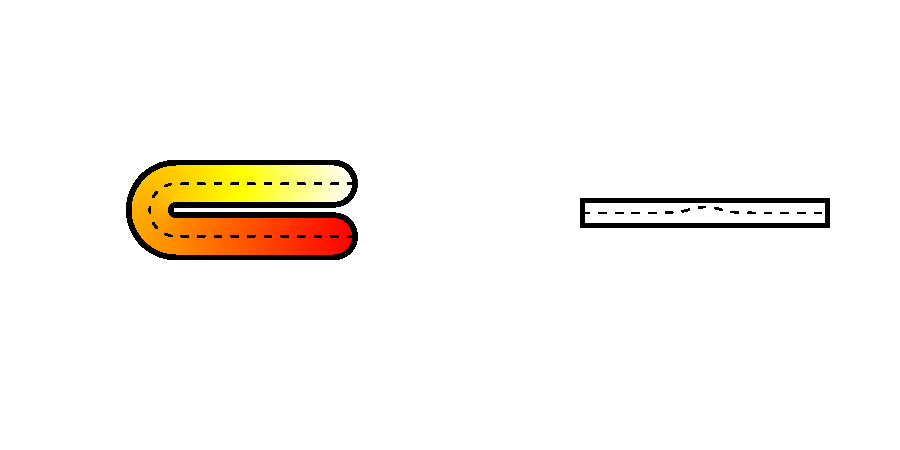
\includegraphics[trim=0in 1.5in 0in 1.5in]{figs/horseshoecentreline.pdf} \\
\caption{The dashed line here gives the centre line that we will map to investigate the smoothness under the \sch transform.}
\label{horseshoecentreline}
\end{figure}


%\begin{figure}
%\centering
%% trim order l b r t
%\includegraphics[trim=1in 1.5in 1in 1.5in]{figs/horseshoecentrelinemapped.pdf} \\
%\caption{The dashed line here gives the centre line that we will map to investigate the smoothness under the \sch transform.}
%\label{horseshoecentrelinemapped}
%\end{figure}

Linear fit onto the horseshoe.
Look at some other shapes that break it.


\section{Simulations}

In the spirit of those simulations carried out in \cite{soap}, a large scale experiment was run and comparison made to those results. We looked at two different test function on the Ramsey horseshoe; first the one described above, and the second with a gradient across the short axis of the horseshoe. This, second, test function can be seen in \fig{ramseyalt}. Table (\ref{simtable}) shows the setup of these experiments, these were run on both test functions.


\begin{figure}
\centering
% trim order l b r t
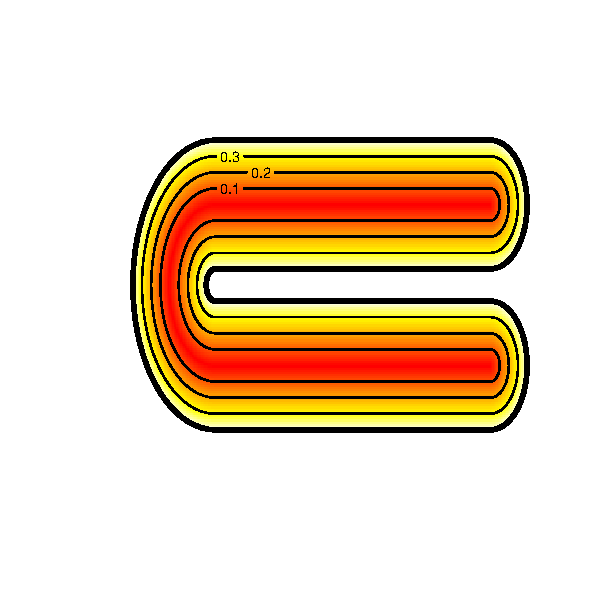
\includegraphics[trim=0in 1.5in 0in 1in]{figs/altramsayhorseshoe.pdf} \\
\caption{Heatmap of the alternate version of the Ramsay horseshoe.}
\label{altramsayshorseshoe}
\end{figure}

\begin{table}[ht]
\begin{tabular}{c c}\\
Sample size & Noise level$^{1}$ \\
\hline
1000 & 0.3 \\
500 & 0.3 \\
250 & 0.3 \\
100 & 0.3 \\
1000 & 0.3 \\
1000 & 0.5 \\
1000 & 1 \\
1000 & 2 \\
\end{tabular}
\caption{Setup for the simulations. $^{1}$Noise level is noise added to the test function from a standard Normal multiplied by the value in this column. }
\end{table}

Again, following in the footsteps of \cite{soap}, the mean squared error between the true function and the fitted model was used to evaluate the model's performance.

For the standard Ramsay horseshoe initial results were better than those for the soap film smoother \fig{ramsaysoapboxplot}.


Table (\ref{ramsayresultstable}) shows the results from the 


\begin{table}[ht]
\begin{tabular}{c c c c}\\
Sample size & Noise level & P-spline MSE (\emph{se}) & Soap MSE (\emph{se}) \\
\hline
\hline
1000 & 0.3 & 0.00412 (0.00112) & 0.00517 (0.00114) \\ 
500 & 0.3 & 0.00505 (0.00144) & 0.00628 (0.00146) \\ 
250 & 0.3 & 0.00875 (0.00392) & 0.0107 (0.00305) \\ 
100 & 0.3 & 0.51 (13.4) & 0.0223 (0.01) \\ 
1000 & 0.5 & 0.0105 (0.00353) & 0.0127 (0.0034) \\ 
1000 & 1 & 0.0242 (0.0108) & 0.0275 (0.00958) \\ 
1000 & 2 & 0.066 (0.0481) & 0.0686 (0.0333) \\ 
\end{tabular}
\label{ramsatresultstable}
\caption{}
\end{table}





\bibliographystyle{plainnat}
\bibliography{sc-refs}



\end{document}
